% !TEX encoding = UTF-8 Unicode
\documentclass[pdftex, a4paper,12pt]{report}

\usepackage[utf8]{inputenc}
\usepackage[T1]{fontenc}
\usepackage[french]{babel}
\usepackage[pdftex]{graphicx}
\usepackage{xcolor}
\usepackage{listingsutf8}
\usepackage{geometry}

\geometry{left=2cm, right=2cm, top=2cm, bottom=2cm}
\newcommand{\HRule}{\rule{\linewidth}{0.5mm}} 
\begin{document} 

\begin{titlepage}

\begin{center}

\includegraphics[width=0.15\textwidth]{./logo_INSA_RN}\\[1cm]    

\textsc{\Large PROJET D'APPROFONDISSEMENT ET D'OUVERTURE}\\[0.5cm]

\HRule \\[0.8cm]
{\LARGE \bfseries COMPAGNON VIRTUEL SOUS ANDROID}\\[0.4cm]

\HRule \\[1.5cm]

\textsc{Institut national des sciences appliquées de Rouen}\\[1.5cm]

% Author and supervisor
\begin{minipage}{0.4\textwidth}
\begin{flushleft} \large
\emph{Rédigé par:}\\
Jitao \textsc{XU}

Chenxin \textsc{LU}
\end{flushleft}
\end{minipage}
\begin{minipage}{0.4\textwidth}
\begin{flushright} \large
\emph{Proposé par:} \\
Alexandre \textsc{PAUCHET}
\end{flushright}
\end{minipage}

\vfill

% Bottom of the page
\textsc{\large ASI}\\
{\large \today}

\end{center}
\end{titlepage}


\section*{Introduction}


Dans le cadre de notre scolarité au sein du département Architecture des Systèmes d’Information (ASI) de l’Institut National des Sciences Appliquées (INSA) de Rouen, nous devons réaliser au cours de notre premier semestre de quatrième année un Projet d’Approfondissement et d’Ouverture (PAO), c’est-à-dire un travail sur plusieurs mois, seul ou en équipe, dans lequel nous pouvons mettre en pratique nos connaissances apprises en cours et/ou apprendre de nouvelles connaissances sur des sujets en rapport avec notre formation.
Nous avons donc tous les deux décidé de nous intéresser à un sujet proposé par M. Alexandre Pauchet : la création d’un compagnon virtuel sous Android. Ce PAO permet d’une part de mettre en application nos acquis en Java de troisième année, et d’autre part de découvrir la conception d’une application mobile sous Android, chose totalement nouvelle pour nous deux.
\pagenumbering{arabic}
\newpage

\section*{Chapitre1}
\section*{1.1 Analsye des besoins}
Le principal but du projet est de développer de nouvelles fonctionnalités sur l'application Compagnon Virtuel déjà existante, notre verision sera version 4.
Avant de commencer le projet, l'application est déjà fonctionnelle, elle propose une interaction avec un personnage animé. Ce dernier est capable d'échanger via reconnaissance vocale et synthèse vocale. L'analyse des requêtes est déportée sur un serveur externe de dialogue intelligent: pandorabots. Le compagnon virtuel s'exprime aussi via des animations. Pendant la préparation du projet, nous avons proposé de réaliser les fonctionnalités suivantes:\\
	\indent- effectuer une recherche dans googlemaps et afficher une carte dans l'application.\\
	\indent- envoyer sms.\\
	\indent- ajouter et supprimer un réveil.\\
	\indent- afficher un calendrier au sein de l'application\\
	\indent- intégrer le processus de gestion de calendrier au chatbot externe.\\
	\indent- afficher le prochain événement dans le calendrier, il est capable de mettre à jour le prochain événement s'il y a une modification dans le calendrier.\\
	
Autrement, nous avons proposé de améliorer l'interface d'utilisateurs de l'application car nous n'étions pas satisfaits avec l'interface d'utilisateur actuelle.

\section*{1.2 Rendus}
En résumé, les rendus demandés sont:\\
    \indent- une application fonctionnelle sous Android,\\
    \indent- un rapport sur le déroulement du projet,\\
    \indent- une documentation du code source,\\
    \indent- un guide utilisateur.\\
\indent Ils doivent être fournis avant la fin du premier semestre de ASI 4.1, afin d'être compabilisés dans la moyenne semestrielle.
\newpage


\section*{Chapitre 2}
\section*{Spécification}
\section*{2.1 Faisabilité du projet}
Dans un premier temps, nous avons suivi un cours sur www.udacity.com pour apprendre la base des connaissances de développer une application sous Android. Ce cours nous permet de développer une simple application, par exemple un compteur de points qui est utilisé dans le match du basket sous Android nous-même. Donc, nous pensons que nous sommes capable de commencer notre PAO.\\\\
\indent Ensuite, nous avons effectué une brève étude bibliographique quant à la faisabilité du développent de fonctionnalités que nous avons proposé. Nous avons trouvé des APIs du développement sous Android. Dans ce cas là, nous pensions que tous les fonctionnalités pouvaient être développés sous Android sans trop de difficulté. \\\\
\indent Concernant la partie de la réponse intelligente, comme les anciens PAOs sur ce sujet, nous avons décidé d'utiliser le Pandorabots, outils Internet permettant d'héberger un grand nombre de fichiers AIML contenant les question/réponses, pour nous aider de réaliser tous les fonctionnalités.
Le choix du IDE a été fait rapidement, nous avons choisi Android Studio qui est un IDE très moderne. \\\\
\indent Notre application peut être fonctionnée sur Android 4.4 ou supérieur avec une connexion Internet permanante.\\

\section*{2.2 Analyse Descendante}
\begin{figure}[h]
\centering
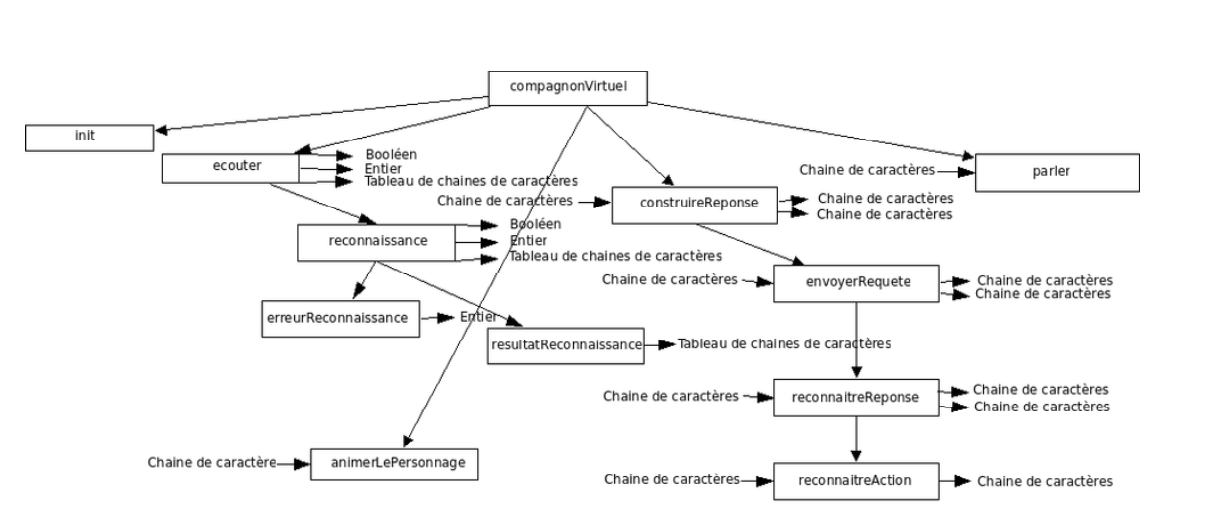
\includegraphics[width=1\linewidth]{analyseDescendante.png}
\caption{Analyse descendante de la version ancienne.\label{fig1}}
\end{figure}



\end{document}